\documentclass[12pt]{article}
\usepackage[margin=.6in]{geometry}
\usepackage{amsmath,amsfonts,amssymb,mathtools}
\usepackage{enumerate}
\usepackage{physics}
\usepackage{graphics,graphicx,epstopdf}
\usepackage[dvipsnames]{xcolor}
\usepackage{float}
\usepackage{hyperref}
\setlength\parindent{0pt}

\newcommand{\R}{\mathbb{R}}
\newcommand{\N}{\mathbb{N}}
\newcommand{\Z}{\mathbb{Z}}
\newcommand{\T}{\mathbb{T}}
\newcommand{\Q}{\mathbb{Q}}
\newcommand{\D}{\mathbb{D}}
\newcommand{\e}{\mathrm{e}}
\newcommand{\C}{\mathbb{C}}

\newcommand{\figlabel}[1]{\textbf{(#1)}}

\newcommand{\comment}[1]{\textsc{\color[rgb]{1,0,0}#1}}

\title{Principal Component Analysis for Semantic Classification \\ AMATH 582 Final Project}
\author{Benjamin Liu, Kelsey Maass, and Riley Molloy}
\begin{document}

% Title/author/abstract
\maketitle
\bigskip

% Abstract
\abstract{Principal component analysis (PCA) and classification by supervised learning are two popular topics in data science today. In this project, we combine techniques from both areas in order to classify news articles based on their word frequency content. We find that we can accurately classify the data by projecting onto a small subset of principal components, reducing the feature space from nearly $10 \,000$ elements to just four. We also compare results from the traditional and robust PCA formulations, and discuss what additional semantic information can be inferred from our results.}


% Sec 1. Introduction and Overview
\section{Introduction and Overview}
Dimensionality reduction is a property which all data scientists look for in their work. It allows for ease and speed in computation and promotes less complexity in many dense problem spaces. Principle component analysis is a standby in dimensionality reduction techniques, grounded in the power and breadth of the singular value decomposition. 

Our work employs the use of PCA to lower the dimensionality of a large set of word-frequency data in five different classes of articles published by the British Broadcasting Corporation (BBC): Business, Sports, Entertainment Politics, and Technology. Each article, considered a single observation, is treated as a vector in the space of words used in every article. Each component of a vector represents the frequency of a given word throughout the article. We look to reduce this large space of words and represent each article with a small number of components, then classify each article as one of the five article types---i.e., we look to learn the semantics of each article in its low-dimensional feature space. This type of analysis is often referred to as ``Latent Semantic Indexing.''

In order to test the validity of our dimensionality reduction, we employ four different supervised learning techniques for classification: Nearest mean, $K$-nearest neighbors, Logistic regression, and a Neural network. We examine the accuracy of the classification for each method and how it varies with the number of principle components used to represent the feature space. 

In addition to PCA, we also employ a variant known as Robust PCA, and classify using its results as well. Robust PCA first separates the original data matrix into two matrices: a sparse matrix and a lower rank matrix. In our application, the sparse matrix should indicate words which are not found in many articles, but are prominent in a few. Thus, the low rank matrix contains fewer outliers  and consists of data on which the traditional PCA procedure should yield better results. 


% Sec 2. Theoretical Background
\section{Theoretical Background}

\subsection{Principal Component Analysis
}
Principal component analysis is a powerful tool for isolating low-dimensional
structure embedded in high-dimensional data. The goal of PCA is to find the best
linear transformation of the data which maximizes the variance in the first principal component direction and in each subsequent orthogonal directions. To perform PCA, we recall the Singular Value Decomposition, or SVD, 
\begin{align} 
A &= U \Sigma V^*,
\label{eq:svd}
\end{align}
which exists for every matrix $A \in \R^{m \times n}.$ We refer to the number of nonzero singular values of a matrix as the \emph{rank} of a given matrix. We refrain from listing otherwise significant information about the SVD in hopes that the reader holds some level of awareness of the relevant theorems and properties. 

We arrange our matrix of data $A \in \R^{ 9635 \times 2225 } $ such that each row represents a different word (or \emph{feature}) and each column represents a different article. We arrange the columns by the classes of articles. In addition, we require this matrix to have rows of mean zero. Since this will not be true of the data initially, we redefine $X$ by subtracting off the mean of each row of $X$, and letting this be the ``new'' data matrix. We then take the SVD of this matrix as in \eqref{eq:svd}.

The matrix $U$ now consists of columns which represent the ordered principle components, $\Sigma$ represents the importance of each singular value with respect to the others, and $V$ represents how each article is projected onto the principle component space. To represent each article $i$ in terms of the determined principle components, we can view each article as $\sigma_i v_i $, where $\sigma_i$ the corresponding singular value from $\Sigma$, and $v_i$ is the $i$-th \emph{row} of $V$. Since we look to reduce the dimensionality of the data, we intend to only examine a small number of principle components; therefore, we look at only the first several components of $v_i$.

\subsection{Robust PCA}
Robust Principle Component Analysis is a variant of PCA which presupposes the data has some low dimensionality suitable for PCA, but with an unknown amount of sparse noise within the data. That is, for the data matrix $A$, we assume that 
$$  A \approx L + S,$$
where $L$ has low rank and $S$ is sparse. To penalize these properties convexly, we consider the formulation
\begin{align}
\min_{L,S} \norm{A-L-S}_{F}^2 + \lambda_1 \norm{L}_* + \lambda_2 \norm{S}_1,
\label{eq:robust_obj}
\end{align}
where $\norm{\cdot}_*$ is the nuclear norm, defined by
\begin{align*}
\norm{\cdot}_* = \norm{\sigma(\cdot)}_1
\end{align*}
where $\sigma$ maps a matrix to a vector of its singular values. Therefore the nuclear norm of a matrix is the sum of its singular values. In addition, $\norm{\cdot}_1$ is the vectorized $\ell_1$ norm, treating $S \in \R^{m \times n}$ as $S \in \R^{mn}.$ The quantity $A - L - S$ is considered an error term, added in for computational stability. The parameters $\lambda_1$ and $\lambda_2$ can be tuned to prioritize low rank in $L$ or sparsity in $S.$ We can now choose one of many available methods for solving convex optimization problems. Our approach is discussed in the Algorithms section of this report. 


\subsection{Classification Methods}
\comment{Kelsey}
% Sec 3. Algorithm Implementation and Development
\section{Algorithm Implementation and Development}

\subsection{Article Data}

Our dataset consists of 2225 BBC articles labeled by topic, including business (510), entertainment (386), politics (417), sports (511), and technology (401). The data, collected for a paper presented at the 2006 International Conference on Machine Learning [1], consists of integer word counts for 9635 distinct words subject to the following pre-processing steps:
\begin{enumerate}
\item Stemming to identify like-words (e.g. fish, fisher, fishing, fishes)
\item Removal of stop words (common words such as: a, about, am, any, are, etc.)
\item Low-count (less than 3) removal
\end{enumerate}

\subsection{Robust PCA}
As mentioned previously, many methods of optimizing \eqref{eq:robust_obj} exist. We chosen to implement a method described in \cite{prox} known as \emph{Alternating direction method of multipliers} (ADMM), or \emph{Douglas Rachford splitting}. The algorithm consists of finding closed form representations of the proximal operators of the nuclear norm and the vectorized 1-norm, and evaluating them iteratively and independently, comparing their results.  

\subsection{Classification Schemes}
\comment{Kelsey addition}

To classify articles in our cross validation set, we first project both datasets onto a subset of the training data’s principal components. Next we compare our classification accuracy as we increase the number of principal components used for the following classification methods:

\subsubsection{Nearest Mean}

For the nearest mean method, we first project the training data onto
the first four principal components and calculate the average projection for each class. To classify new articles, we assign the label of the closest mean projection.

\subsubsection{K-Nearest Neighbors (KNN)}

The K-nearest neighbors algorithm classifies new articles by
finding their K nearest neighbors and assigning the label shared by the most neighbors. For our article classification, we let $K = 5$.

\subsubsection{Logistic Regression}

Logistic regression classifies articles by first drawing linear decision
boundaries between the classes (one-vs-all) that maximize the log-likelihood of the probabilities that the training articles belong to their respective classes. The final label is chosen from the class with the highest probability.

\subsubsection{Neural Network}

To classify with neural networks, we first build a network with three
layers: input, hidden, output. We then train the network to minimize a cost function on the training data and assign classes to new articles by choosing the class with the highest output value.

\subsubsection{Support Vector Machine}

\comment{ben's results}

% Sec 4. Computational Results
\section{Computational Results}
\comment{Poster materials}

\subsection{PCA and Robust PCA}
\begin{figure}[H]
\centering
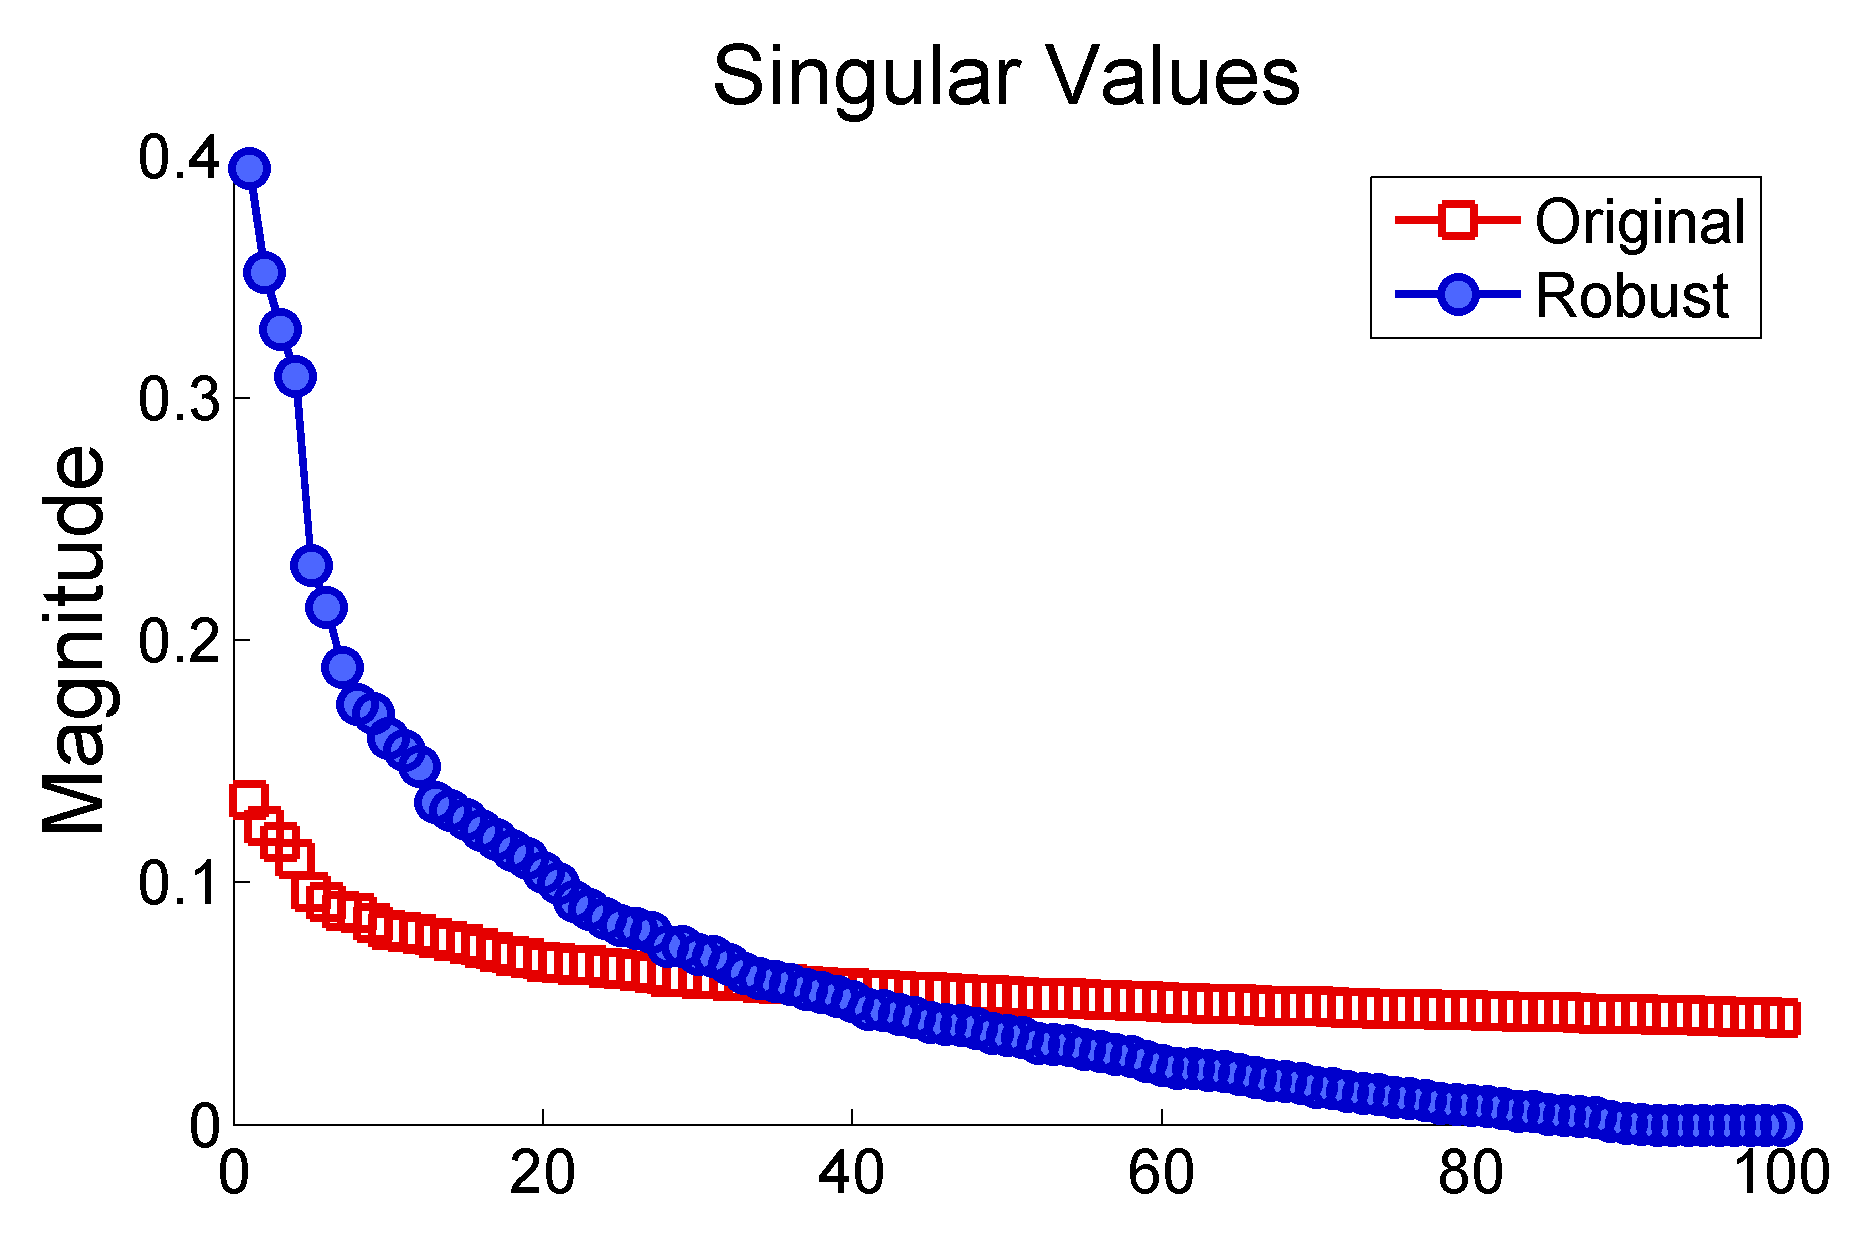
\includegraphics[width=.6\textwidth]{figures/singularvaluescompare}
\end{figure}

\subsection{Classification}

% Sec 5. Summary and Conclusions
\section{Summary and Conclusions}
\comment{Ben}

\begin{thebibliography}{4}
\bibitem{clustering} D. Greene and P. Cunningham, \emph{Practical Solutions to the Problem of Diagonal Dominance in Kernel Document Clustering}, Proc. ICML, 2006.
\bibitem{rpca} Y. Ma, E. J. Candes, X. Li, and J. Wright. \emph{Robust Principal Component Analysis?} Technical report, Stanford University , Stanford CA, 2009.
\bibitem{nathan} J. N. Kutz. \emph{Data-Driven Modeling \& Scientific Computation: Methods for Complex Systems and Big Data.} Oxford University Press, 1 st edition, 20013.
\bibitem{prox} N. Parikh, S. Boyd, \emph{Proximal Algorithms.} Foundations and Trends in Optimization, Vol. 1, No.3, 2013.
\end{thebibliography}

\newpage
% App A. MATLAB functions used and brief implementation explanation
\section*{Appendix A: MATLAB Functions}

\paragraph{ind = knnsearch(Xtrain,Xtest,k)} Finds the \textbf{k} elements of \textbf{Xtrain} that are nearest to \textbf{Xtest}, and returns the indices of these elements in \textbf{ind}.

\paragraph{svmtrain}

\paragraph{svmdecision}

% App B. MATLAB codes
\section*{Appendix B: MATLAB Codes}

All of our code can be accessed {\color{blue}\href{https://github.com/kels271828/582FinalProject.git}{here}}.

% App C. (optional) Any algebraically intense calculations (long and drawn out calculations that have no business in Sec 2)
% \section{Appendix C}

\end{document} 